\section{ Related Work } 
\subsection{Motion Primitives}

Motion primitives is a well defined concept for representing modular and
re-usable skills in robotics. Motion primitive can be considered as
elementary building blocks for skill representation \cite{kruger_learning_2010}.
Motion primitives are commonly used for representing and learning skills in
robotics.

There is generally two distinct approaches to represent motion primitives, one
at the trajectory level and the other at the symbolic level \cite{argall_survey_2009}.
One of the early techniques in the trajectory level approaches was as a spline
by \cite{ude_trajectory_1993}. The other most common method is to represent
motion primitives as a  probabilistic representation \cite{calinon_robot_2009}.
\acrfull{gmm} is used to encode motion primitives through probabilistic
representation. \acrshort{gmm} allowed autonomous and incremental construction
of the motion primitives. This was beneficial for \acrshort{lfd}. \acrfull{hmm}
is used to encode motion primitives. In \acrshort{hmm} the motion primitives
are represented as a single multivariate Gaussian Distribution.
\cite{paraschos_probabilistic_2013} introduced the concept of probabilistic
movement primitives (Promotion primitives) as generalistic framework for
representing and learning motion primitives.

A popular alternative to this approach has considered modelling the intrinsic
dynamics of motion \cite{schaal_nonlinear_2000} . This approach was advantageous
for \acrshort{lfd} as it was time-independent and can be modulated to produce trajectories
with similar dynamics in area of workspace not covered during learning. One of
the drawbacks of the trajectory based techniques was that it lacks cognitive
sense \cite{aein_toward_2013}. These
drawbacks are also been addressed in current research activities like
\cite{manschitz_learning_2015} where the transition between
the motion primitives are also being learned to execute complex tasks.

In symbolic representations a compact descriptions of motion primitives is defined, but the
execution details are not included. A large body of work uses symbolic
representation for encoding motion primitives (\cite{muench_robot_1994},
\cite{friedrich_robot_1996}, \cite{pardowitz_incremental_2007}).
\cite{alissandrakis_approach_2005} encoded human motions as
pre-defined postures, positions or configurations. \cite{aein_toward_2013} creates a library
of motion primitives. In a more recent work by \cite{andersen_using_2014} the skill
based framework is used to learn predefined
skills. The skills are made of combinations of motion primitives. The configuration
parameters of the motion primitives are learnt by demonstrations. The paper proposes an
approach to represent skill for learning inside a skill based framework.
But in the above work the representation of motion primitives in a skill based framework is
not well defined.

\subsubsection{Proposed Motion Primitive }
\label{sec:Proposed motion primitive}
We represent motion primitives as foundation blocks
for a robot to complete a skill. For example consider a "pick up skill" can be
executed using combinations of "move" Motion primitive. So a \textit{pick up screw}
skill gets fragmented as \textit{move arm camera pose} + \textit{move arm grasp pose} + \textit{move
arm place pose}. Which motion primitives are available to a robot depends on the hardware
specification of the robot.

Each motion primitives has a pre-condition and post-conditions to ensure and verify a proper
functioning. Using \acrshort{lfd} we try to learn the post-condition(goal) of the motion primitives. The
motion primitives in our framework consist of a teaching part and an execution phase, as
illustrated in Figure \ref{motion primitive} (extended from \cite{bogh_does_2012} and \cite{andersen_using_2014})
The motion primitive using this approach is well suited for the skill
based framework as explained in \cite{pedersen_robot_2015}. 
\begin{figure}[htp] \centering
    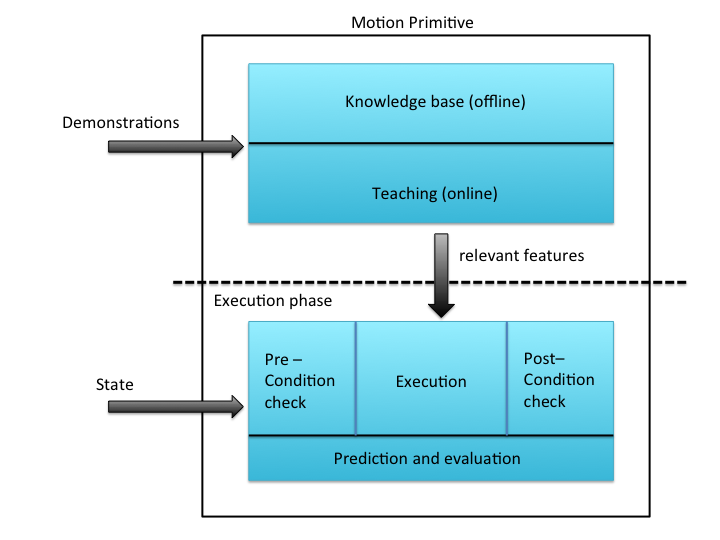
\includegraphics[scale=0.5]{images/motion_primitive_color.png}
    \caption[General structure of a motion primitive]{Proposed general
    structure of a motion primitive. A motion primitive consist of Learning
Phase and Execution Phase.} \label{motion primitive} \end{figure}

The motion primitive as shown in figure \ref{motion primitive} consist of two parts 
the learning part and the execution part.
In the learning part the demonstrations are taken as an input and the relevant features are 
extracted. This extracted features are then fed to the execution part.
The execution part is represented as a combination of pre and post conditions of features.
Based on the relevant features the execution phase predicts the post conditions 
and executes  the motion primitive.
In section \ref{sec:Learning motion primitive} the mathematical formulation of the 
motion primitive is discussed in details.

\subsection{Goal Based Learning from Demonstration}
A large body of work uses
goal based or plan based representation of learning\\
(\cite{friedrich_robot_1995},
\cite{nicolescu_natural_2003}, \cite{csibra_obsessed_2007}, \cite{demiris_prediction_2007},
\cite{veeraraghavan_teaching_2008}, \cite{lee_effective_2009}, \cite{hommel_action_2009}, \\ 
\cite{abdo_learning_2013}). 
The majority of the work in these try to infer the underlying goals and intent of
the demonstrator. The terms goals and intent are used interchangeable; but
goal refers to the immediate desirable state while intent refers to longer term
desirable state. \cite{tomasello_understanding_2005} defines intent as \textit{" a plan of
    action the organisam chooses and commits itself to the pursuit of a goal,
an intention thus includes both a means(action plan) as well as goal"}(p676).

The idea of learning goals is inspired by learning techniques in humans. It has
been studies that humans show a strong and early indication to interpret
observed behaviours of others as goal directed actions. This is termed as
'teleological obsession' \cite{ csibra_obsessed_2007} . They argue this
'teleological obsession' serves for on-line prediction and social learning.

The problem of recognizing goals and intentions of the action can be formulated
as a problem of model matching. The agent which is observing deploys sensors,
each reporting its observations of the state. Based on the state observations, two
approaches are available for analysis \textit{descriptive} and \textit{generative}
\cite { demiris_prediction_2007}

In \textit{generative} approach the observed states are mapped into a latent(hidden)
space. The latent space is usually of lower dimension than the observation
space. The main problem of inferring in the observation space is the
dimensionality of the space. So by reducing the observations to latent space
learning is made on smaller dimensions. Generative model is highly popular in
machine learning community and robotics community (\cite{buxton_learning_2003}, \cite{bishop_pattern_2006}
, \cite{calinon_robot_2009})

In contrast, in the  \textit{descriptive} approach, the patterns are characterised by
extraction of a number of low level features, and to use the set of
restrictions of the features level(\cite{isham_introduction_1981}, \cite{jain_deformable_1998}, 
\cite{abdo_learning_2013}). The
observer agent subsequently matches the observed data against pre-existing
representations and depending on what the task is show generates the action
corresponding to their representations. Pre -existing representations can have
associated data that label these representations with the goals, beliefs and
intentions that underlie in the demonstrations. This approach corresponds to the \acrfull{tec}
method for intention interpretation by \cite{csibra_obsessed_2007}. \acrshort{tec} was formulated
to provide an alternative prespective that allows to take intentions and the
goal directed nature of action into consideration. \acrshort{tec} explains how human
learning works; basically how human action is anticipatory in nature, how
anticipation emerge from experience and, how anticipation comes to regulate
human behaviour.

Our work is an extension of the \textit{descriptive} approach of learning. We also learn
using the restircted feature space.

\subsubsection{Proposed Expert Knowledge Base} 
A recent work by \cite{abdo_inferring_2014} leverages feedback from experts to create a
recommendations and use this recommendations to recommend features for actions.
Our approach advances over \cite{abdo_inferring_2014}, by creating  a more structured
knowledge base . The expert knowledge base used in the previous is not
structured. In this work we try to create a more structured generic framework
based on effect metrics concept. The expert knowledge base is explained in 
details in the section \ref{sec:Learning motion primitive}.

\subsection{Recommender system in Robotics}
Use of the recommender system in robotics is a very recent affair. Recommender
system is a special branch in machine learning which specializes in determining
the user preferences, based on previous activites of the user. It then uses
this user preferences to predict products(movies, videos, news etc) which the
user will like to see or purchase. Recommender systems are broadly classified
into two types \textit{Content Based Recommender System} and
\textit{Collabrative Recommender System} \cite{bobadilla_recommender_2013}. The use of recommender system in
robotics is relative a new approach. The first to use was by \cite{matikainen_model_2012},
who used it to the model recommendation problem. They tried to recommend based
on previous history which machine learning algorithm to use for a specific
image processing situation. In \cite{matikainen_multi-armed_2013} they tried to
solve the n-bandit problem of selecting food floor coverage statistics using
recommender system.

Further Recommender system was used to learn user preferences of the users for
doing daily chorus for robots. \cite{abdo_collaborative_2014} and
\cite{abdo_robot_2015} tried to learn user preferences concerning a given
tasks using small number of known preferences. Using recommender system they
enable robots to predict user preferences with respect to tidying up objects in
containers,  such  as  shelves  or  boxes.



